\label{sec:extension}
Inherently, there is no unique "ground-truth" image that conforms to the given semantic layout. For example, given a semantic layout of a car, we can synthesize a black, red, or white car and it might be facing front or back. Our CRN is able to generate diverse images explicitly.

In order to generate $k$ images from our network, we simply change the number of feature channels in the final layer from $3$ to $3k$. Every three feature maps can form an image, totally $k$ images. With $k$ output images, we also need to adjust our loss function. We need a loss function that measures the distance between a reference image in the training data and $k$ generated images. Intuitively, we should not penalize as long as the reference is close to one of $k$ output images. Let $g_u(L,\theta)$ denote the $u$-th image the network synthesize. The loss $\lL(I,L;\theta)$ for our CRN with $k$ output images would become \cite{Lee2016},

\begin{equation}
\min_u{\sum_l{\lambda_l\| \Phi_l(I)-\Phi_l(g_u(L;\theta))\|_1}}.
\label{eqn:diversity_loss_1}
\end{equation}
This loss encourage diversity in the output images, because having the same output images does not help reduce the loss. We only need one of them for comparison. This loss is similar to k-means clustering loss and the centroid is unlikely to collide.

Furthermore, the loss (\ref{eqn:diversity_loss_1}) can be improved as we could construct up to $k^c$ different images from just $k$ output images: for each class out of $c$ semantic classes, we can choose one $k$ images to fill the content of the regions of that class. However, it is computationally intractable to explicit compute $k^c$ images.

In fact, computing the loss between the reference image and $k^c$ constructed images can be computed efficiently, semantic classes are sperable during construction. Intuitively, as long as one of $k$ images has similar output with the reference image in the areas of that semantic class, we should not penalize. Therefore, we can have a loss that sum up the per-class losses:
$$
\sum_{p=1}^c{\min_u{\sum_l{\lambda_l\|mask(L,p,l) \odot \left(\Phi_l(I)-\Phi_l(g_u(L;\theta))\right)\|_1}}},
$$
where $mask(L,p,l)$ is a mask image $M$ with the same shape of $\Phi_l$. Suppose $M$ has shape $m'\times n' \times w'$ and let $L'$ be the resized semantic layout of $L$ with size $m'\times n'\times c$. Then $M_{i,j,z}=L'_{i,j,p}$ for all $z$. $M$ eliminates penalty in regions where the semantic class is not $p$.

\begin{figure}[H]
  \centering
  \begin{tabular}{@{}c@{\hspace{0.5mm}}c@{}}
  \includegraphics[width=0.235\textwidth]{figures/diversity/1.png}&
  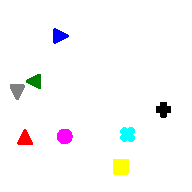
\includegraphics[width=0.235\textwidth]{figures/diversity/2.png}\\
  Output A& Output B\\
  \end{tabular}
  \caption{diversity.}
\label{fig:diversity}
\end{figure}
